\documentclass[
    11pt,
    parskip=half,
    abstract=on,
]{scrreprt}
\usepackage[a4paper, tmargin=2.54cm, bmargin=2.54cm, lmargin=18mm, rmargin=18mm]{geometry}

\setcounter{tocdepth}{1}
\renewcommand{\figurename}{Figure}
\renewcommand{\listfigurename}{List of Figures}

\usepackage{graphicx}
\graphicspath{{figures/}}

\usepackage{array}
\usepackage[square,sort,comma,numbers]{natbib}
% \usepackage[comma,authoryear]{natbib} % Use to validate duplicate references
\usepackage{booktabs}       % professional-quality tables
\usepackage{pgfplotstable}  % read csv tables
\pgfplotsset{compat=1.14}
\usepackage{longtable}
\usepackage{tabu}
\usepackage[utf8]{inputenc} % allow utf-8 input
\usepackage[T1]{fontenc}    % use 8-bit T1 fonts
\usepackage{hyperref}       % hyperlinks
\usepackage{url}            % simple URL typesetting
\usepackage{amsfonts}       % blackboard math symbols
\usepackage{amsmath}
\usepackage{nicefrac}       % compact symbols for 1/2, etc.
\usepackage{microtype}      % microtypography
\usepackage{xcolor}         % colors
\usepackage{changepage}
\usepackage[printonlyused]{acronym}
\usepackage{subcaption}
\usepackage[ruled, vlined, linesnumbered]{algorithm2e}
\usepackage{datetime}
\usepackage{pdfpages}

\usepackage{soul} % Used to highlight text

\definecolor{hypecol}{HTML}{0875b7}
\hypersetup{%
    colorlinks,
    linkcolor={hypecol},
    citecolor={hypecol},
    urlcolor={hypecol}
}


\NewDocumentCommand{\thesischapter}{o m m}{%
   \IfNoValueTF{#1}
     {\chapter[#2]{#2\origtitle{#3}}}
     {\chapter[#1]{#2\origtitle{#3}}}%
}
\newcommand\origtitle[1]{\\
  \parbox{\textwidth}{\normalsize\vspace*{2\baselineskip}#1}}

\newdateformat{monthyeardate}{%
  \monthname[\THEMONTH] \THEYEAR}

\begin{document}

\includepdf[pages={1}]{chapters/front-and-back-cover/front-and-back-cover.pdf}
\includepdf[pages={2}, angle=90]{chapters/front-and-back-cover/front-and-back-cover.pdf}
\thispagestyle{empty}
\begin{titlepage}
    \begin{center}
        \large{\textbf{\textsf{NOVA Information Management School}}}
        \vspace{0.2cm}\\
        \large{\textbf{\textsf{Instituto Superior de Estatística e Gestão de Informação}}}
        \vspace{0.2cm}\\
        \large{Universidade Nova de Lisboa}
        \vspace{3.5cm}\\

        \LARGE{\textbf{\textsf{%
            The Role of Synthetic Data in Improving Supervised Learning
            Methods: The Case of Land Use/Land Cover Classification
        }}}
        \vspace{1cm}\\
        \large{by}
        \vspace{1cm}\\
        \large{João Pedro Martins Ribeiro da Fonseca}
        \vspace{3.5cm}\\
        \large{\textsf{Doctoral Thesis presented as partial requirement for
        obtaining the PhD in Information Management}}
        \vspace{3cm}\\
    \end{center}
	
    \textbf{\textsf{Supervisor:}} Professor Fernando Bação, PhD

    \begin{center}
        \vspace{4cm}
        \monthyeardate\today
    \end{center}
	
\end{titlepage}

\newpage

\pagenumbering{roman}
\setcounter{page}{1}
\chapter*{Statement of Integrity}

I hereby declare having conducted this academic work with integrity. I confirm
that I have not used plagiarism or any form of undue use of information or
falsification of results along the process leading to its elaboration. I
further declare that I fully acknowledge the Rules of Conduct and Code of
Honor from the NOVA Information Management School.\\

Lisbon, \usdate\today
\vspace{-.5cm}

\begin{minipage}{0.3\textwidth}
    \centering 
    \includegraphics[width=0.6\textwidth]{jfonseca-signature.png}\\
    \vspace{-1cm}
    \rule{\textwidth}{.3pt}\\
    \large{João Fonseca}
\end{minipage}
\vspace{0.3cm}



\chapter*{Dedication}

To my parents, José Manuel and Maria de Lurdes Fonseca. 

\chapter*{Acknowledgements}

MIT Portugal - funding

Fernando Bacao - advisor

Georgios Douzas - discussions, tips and help on technical implementations
throughout the research work

English professor from NOVA IMS - proofreading multiple chapters of this
dissertation

My parents, José Manuel and Maria de Lurdes, my siblings, Hugo and Inês, my
grandmother, Teresa, my girlfriend, Yasmina El Fassi and my brother-in-law,
Hugo Nunes. 

My friends, Pedro Rodrigues, Francisco Martins, Miguel Meco,
Andrew Bell, Rafaela Henriques, Margarida Saragoça, Manvel Khudinyan,
Francisco Braga, Miguel Portas, Mari Reyes, Ana Vieira, Ana Correia, Oumaima
Derfoufi

My secondary school's biology teacher, Regina Lucena, who taught us life
skills well beyond the courses' syllabi, and tremendously inspired me towards
a research-oriented path (without me realising it).

Professor Marco Painho and my friends from the doctoral program, Vicente Tang,
Maria Anastasiadou and Darina Vorobeva

\chapter*{Abstract}

\begin{adjustwidth}{30pt}{30pt}

    In remote sensing, Land Use/Land Cover (LULC) maps constitute important
    assets for various applications, promoting environmental sustainability
    and good resource management. Although, their production continues to be a
    challenging task.  There are various factors that contribute towards the
    difficulty of generating accurate, timely updated LULC maps, both via
    automatic or photo-interpreted LULC mapping. Data preprocessing, being a
    crucial step for any Machine Learning task, is particularly important in
    the remote sensing domain due to the overwhelming amount of raw, unlabeled
    data continuously gathered from multiple remote sensing missions. However
    a significant part of the state-of-the-art focuses on scenarios with full
    access to labeled training data with relatively balanced class
    distributions. This thesis focuses on the challenges found in automatic
    LULC classification tasks, specifically in data preprocessing tasks.  We
    focus on the development of novel Active Learning (AL) and imbalanced
    learning techniques, to improve ML performance in situations with limited
    training data and/or the existence of rare classes. We also show that much
    of the contributions presented are not only successful in remote sensing
    problems, but also in various other multidisciplinary classification
    problems. The work presented in this thesis used open access datasets to
    test the contributions made in imbalanced learning and AL. All the data
    pulling, preprocessing and experiments are made available at
    \href{https://github.com/joaopfonseca/publications}{https://github.com/joaopfonseca/publications}.
    The algorithmic implementations are made available in the Python package
    \textit{ml-research} at
    \href{https://github.com/joaopfonseca/ml-research}{https://github.com/joaopfonseca/ml-research}.

\end{adjustwidth}

\vspace{.5cm}
\textbf{Keywords:} LULC classification; Active Learning;
Imbalanced Learning; Synthetic Data; Oversampling; 

\vspace{.5cm}
\textbf{Sustainable Development Goals (SDG):} 

\includegraphics[width=.15\linewidth]{sdg13}
\includegraphics[width=.15\linewidth]{sdg15}

{\parskip=0pt \hypersetup{linkcolor=black}

\tableofcontents

% \chapter*{List of Acronyms}
% 
% \begin{acronym}[ICANN]
%     \acro{lulc}     [LULC]  {Land Use/Land Cover}
%     \acro{ml}       [ML]    {Machine Learning}
%     \acro{al}       [AL]    {Active Learning}
%     \acro{smote}    [SMOTE] {Synthetic Minority Oversampling Technique}
% \end{acronym}
% \addcontentsline{toc}{chapter}{List of Acronyms}

% LIST OF FIGURES
\listoffigures
\addcontentsline{toc}{chapter}{List of Figures}

% LIST OF TABLES
\listoftables
\addcontentsline{toc}{chapter}{List of Tables}
\pagebreak
}


% MAIN THESIS
\setcounter{page}{1}
\pagenumbering{arabic}
\chapter{Introduction}
\graphicspath{{figures/introduction/}}

% Data availability, satellite images
Accurate LULC maps constitute a unique resource for a variety of applications.
Its applications range from environmental monitoring, land change detection,
and natural hazard assessment to agriculture and water/wetland
monitoring~\cite{Khatami2016}. However, the production of LULC maps often
require the involvement of multiple photo-interpreters with specialized
skills, making the process expensive and time-consuming and unsuitable for
operational LULC mapping over large areas~\cite{Douzas2019rs}. Therefore, the
manual production of LULC maps are often outdated by the time they are
completed, limiting its value to the analysis past conditions in the area of
interest.

An alternative method to address the limitations found in the
photo-interpreted approach to produce LULC maps is automated mapping. This
method uses remotely sensed data, especially multi and hyper-spectral images,
to train ML algorithms to automatically detect the different LULC classes.  To
do this, the usage of recent supervised learning techniques seems to be a
promising path to achieve reliable and updated
maps~\cite{tewkesbury2015critical}. However, the practical application of this
approach is hampered by various limitations: 

\begin{enumerate}
    \item Human error. The quality of the classifiers produced is heavily
        dependent on the quality of its training data. In this case, the
        training dataset is extracted from manually labeled land cover patches
        using typically satellite imagery. The target LULC map's minimum
        mapping unit, as well as the quality of orthophotos and satellite
        images being used are some of the factors that may lead to label noise
        in the training data~\cite{Pelletier2017}.
    \item High dimensionality. The high dimensionality of multi and
        hyper-spectral images contain useful information to improve ML
        classification tasks. However, it also introduces an additional layer
        of complexity and redundancy in classification~\cite{Stromann2020}. If
        the training data is not large enough, it may cause the classification
        task to be affected by the curse of dimensionality.
    \item Class separability. Some LULC classes sometimes contain overlapping
        spectral signatures which makes the separation of the two classes
        particularly challenging in some cases~\cite{Alonso-Sarria2019}.
    \item Infrequent LULC classes. Depending on the region of study, some land
        cover classes may be more or less frequent when compared to other
        regions~\cite{Feng2018}. However, the accurate identification of rare classes
        is often equally or more important than the identification of the
        remaining classes. This problem is known, in ML community, as
        imbalanced learning. As an example, the classification of a desert
        region with 3 classes of interest, bare soil, urban and water, would be
        an imbalanced learning problem. In this case, a classifier that would
        predict bare soil for the entire area of study would have very high
        overall accuracy scores but would not be useful.
    \item Scarcity of labeled data. The increasing number of remote sensing
        missions in the past decades are generating large amounts of high
        quality data. However, only a small portion of this data has some sort
        of LULC ground truth and can be used for supervised learning. In these
        scenarios the production of automated LULC maps is particularly
        challenging and involves the usage of techniques that are able to
        leverage information from both labeled and unlabeled data and
        simultaneously maximize the value of the data annotation
        process~\cite{Simeoni2020}.
\end{enumerate}

The latter two challenges, imbalanced learning (\textit{i.e.}, infrequent LULC
classes) and scarcity of labeled data, are the focus of this thesis. However,
these two challenges may be addressed in various different ways.

The asymmetry frequently found on LULC class distributions affects the
performance of ML classifiers. In this scenario, during the ML classifier's
learning phase, the minority classes contribute less to the minimization of
accuracy, the typical objective function, biasing the classifier towards the
most frequent classes. The possible approaches to deal with imbalanced
learning can be divided into three main groups~\cite{Fernandez2013}: 

\begin{enumerate}
    \item Cost-sensitive solutions. These methods use a cost matrix to adjust
        the misclassification cost to benefit the minority classes.
    \item Algorithmic-level solutions. These methods introduce algorithmic
        solutions to improve the learning process on the minority classes. 
    \item Resampling solutions. They modify the training data to balance the
        class distribution by removing observations from the majority
        class(es) or adding observations belonging to the minority class(es).
\end{enumerate}

The latter set of methods, resampling solutions, benefit from their
simplicity. This type of approaches do not require domain knowledge to define
a cost matrix and dispense the usage of specialized classifiers. These methods
can be further divided into (1) Oversampling, where an algorithm generates
artificial observations belonging to the minority class, (2) Undersampling,
where an algorithm removes observations belonging to the majority class or (3)
Hybrid approaches, which combine oversampling and undersampling together. In
this thesis, we will focus on oversampling methods and generalize these as a
corner case of augmentation methods for tabular data in later chapters. In
Section~\ref{sec:data_augmentation} this topic is discussed to a greater
extent.

The second challenge this thesis focuses on is the implementation of useful ML
algorithms in environments with scarce availability of labeled data. There are
three different types of techniques to address this problem, which fall in
between supervised and unsupervised learning:

\begin{enumerate}
    \item Semi-supervised Learning. Uses both labeled and unlabeled data in
        the training phase to improve the classifier's
        performance~\cite{ouali2020overview}. It pushes the decision
        boundaries of classifiers to regions with lower density of
        observations while maximizing the performance over the labeled
        training dataset~\cite{chapelle2009semi}.
    \item Self-supervised Learning. Uses unlabeled data to perform
        secondary/pretext tasks to learn representations of the input
        space~\cite{grill2020bootstrap}. These methods typically use neural
        network architectures~\cite{liu2021self}.
    \item Active Learning. Iteratively samples the most
        informative/representative observation out of a pool of unlabeled data
        in order to be labeled and included into the training
        dataset~\cite{budd2021survey}. This approach attempts to optimize the
        classifier's performance with as least data as possible.
\end{enumerate}

The latter method, Active Learning, benefits from the possibility of including
different techniques into its pipeline, including the former two. It is
therefore one of the main focus of this thesis. In
Section~\ref{sec:active_learning} this topic is discussed to a greater extent.

\section{Data Augmentation}~\label{sec:data_augmentation}

Data Augmentation methods expand the training dataset by introducing new and
informative observations~\cite{Behpour2019}. The production of artificial data
may be done via the introduction of perturbations on the
input~\cite{Zhong2020}, feature~\cite{DeVries2017} or output
space~\cite{Behpour2019}. Data Augmentation methods may be divided into
Heuristic and Neural Network-based approaches~\cite{Shorten2019}. In addition,
they may also be distinguished based on its data generation policy, whether
local (considers a local/specific subset of the dataset) or global (considers
the overall distribution of the training dataset).
Figure~\ref{fig:data_augmentation_taxonomy} shows the general taxonomy of
Heuristic Data Augmentation methods. Finding the appropriate Data Augmentation
method generally depends on the domain~\cite{DeVries2017}, although some
studies discuss which methods are more appropriate according to the
domain~\cite{Shorten2019, Iwana2021, Wong2016}.

\begin{figure}[ht]
	\centering
	\includegraphics[width=.5\linewidth]{data_augmentation_taxonomy}
    \caption{%
        Schema containing a general Heuristic Data Augmentation taxonomy.
    }~\label{fig:data_augmentation_taxonomy}
\end{figure}

Heuristic approaches attempt to generate new and relevant observations through
the application a predefined procedure, usually incorporating some degree of
randomness~\cite{Kashefi2020}. Since these methods typically occur in the
input space, they require less data and computational power when compared to
Neural Network methods. Neural Network approaches, on the other hand, map the
original input space into a lower-dimensional representation, known as the
feature space~\cite{DeVries2017}. The generation of artificial data occurs in
the feature space and is reconstructed into the input space. Although these
methods allow the generation of less noisy data in high-dimensional contexts
and more plausible artificial data, they are significantly more
computationally intensive. Considering the scope of this thesis, the
computational power available for this experiment and the breadth of datasets
used in the different experimental procedures, we will focus on
domain-agnostic heuristic data augmentation methods.

While some techniques may depend on the domain, others are domain-agnostic.
For example, Random Erasing~\cite{Zhong2020}, Translation, Cropping and
Flipping are image data-specific augmentation methods. Other methods, such as
most of the variants of the Synthetic Minority Oversampling TEchnique
(SMOTE)~\cite{Chawla2002}, may be considered domain agnostic. However, SMOTE
methods were originally developed as oversamplers, whose goal is to balance
the class frequencies of the target variable in the training dataset and
address the class imbalance bias. Therefore, oversampling methods may be
considered a subset of Data Augmentation. Data Augmentation strategies may
follow varying augmentation strategies, which does not necessarily depend on
the target class distribution. An example of the differences among general
data augmentation and oversampling generation strategies is shown in
Figure~\ref{fig:augmentation_strategies}.

\begin{figure}[ht]
	\centering
	\includegraphics[width=.6\linewidth]{augmentation_strategies}
    \caption[Examples of data augmentation Strategies.]{%
        Examples of data augmentation Strategies. The salmon-colored bars
        represent artificial data using the normal oversampling (center group) and
        an example of augmentation (right group) strategies.
    }~\label{fig:augmentation_strategies}
\end{figure}

The simplest approach found in the literature is randomly duplicating existing
training observations. As a non-informed data generation method, although
simple to implement, it increases the risk of overfitting and generally
performs worse than other informed heuristic
methods~\cite{Douzas2019rs}.

The SMOTE method generates artificial data via the linear interpolation
between a random observation and one of its $k$-nearest neighbors (also
randomly selected)~\cite{Chawla2002}. Although simple and effective, it also
contains several limitations which motivated the development other variants,
discussed below. Specifically, its selection mechanism does not consider the
global structure of the dataset while its generation mechanism introduces
little variability into the training dataset~\cite{Douzas2019}.
Borderline-SMOTE (B-SMOTE)~\cite{Han2005} improves the selection mechanism by
attributing a larger importance to the observations closer to the decision
boundaries. The selected observations are used to run the SMOTE method in
order to produce better defined decision boundaries. A more recent improvement
of the selection mechanism is K-means SMOTE (K-SMOTE)~\cite{Douzas2018}. This
method uses a clustering-based approach to overcome imbalances between and
within classes, while considering the densities of each region of the input
space.

\begin{figure}[ht]
	\centering
	\includegraphics[width=.4\linewidth]{smote_vs_gsmote}
    \caption[Examples of data generation using SMOTE and G-SMOTE\@.]{%
        Examples of data generation using SMOTE and G-SMOTE\@. In this
        example, both G-SMOTE's deformation and truncation parameters assume
        values around $0.5$.
    }~\label{fig:smote_vs_gsmote}
\end{figure}

G-SMOTE~\cite{Douzas2019} modifies SMOTE's generation mechanism. Instead of
generating an observation as a linear combination between 2 others, it
generates observations within an hypersphere defined using the selected
observation as its center and one of its nearest neighbors as its boundary.
The hypersphere contains two hyperparameters, the truncation and deformation
factors, which limit the area of the hypersphere. The difference between SMOTE
and G-SMOTE is shown in Figure~\ref{fig:smote_vs_gsmote}.

\section{Active Learning}~\label{sec:active_learning}

Supervised ML algorithms typically perform well in contexts where labeled data
is abundant and accessible. However, in a practical setting, finding this data
is frequently a challenging task. Depending on the domain, collecting large
volumes of data may not be feasible since the labeling of such data becomes
labor and time intensive and may involve domain experts throughout the
process~\cite{Cao2020}. AL maximizes a classifier's performance while
annotating as least observations as possible. It assumes that observations
within the same dataset have a different contribution to the training of ML
classifiers~\cite{Ren2021}. Consequently, the data annotation cost can be
minimized via the annotation of the most valuable observations within an
unlabeled input space. The goal is to iteratively maximize the classification
performance of ML algorithms while minimizing the required amount of training
data to reach a certain performance threshold~\cite{Shrivastava2021}. It
allows the implementation of ML classifiers with a good performance and
minimal effort when compared to randomly selecting data or labeling the entire
unlabeled dataset~\cite{Ren2020}. Therefore, it addresses the labeling problem
in scenarios with a limited budget, time, or availability of labeled data. 

AL methods may be divided into 2 different stages, initialization and
iteration. Figure~\ref{fig:al_initialization} shows a diagram that represents
the typical AL initialization. Assuming the AL task is initialized without any
previously labeled data, it is typically composed of 3
steps~\cite{Fonseca2021}: 

\begin{enumerate}
    \item Collection of an unlabeled dataset, where the procedure depends on
        the domain of application.
    \item Selection of an initial data subset. Typically, when there is no a
        priori labeled dataset, the initial data subset is randomly picked
        from the unlabeled dataset.
    \item Data labeling. The supervisor is presented with the data subset,
        where its goal is to label each observation. Some of the research
        refers to the supervisor as the oracle~\cite{Yoo2019, Aghdam2019}.
\end{enumerate}

\begin{figure}[ht]
	\centering
	\includegraphics[width=.35\linewidth]{al_initialization}
    \caption{%
        Diagram depicting an AL initialization.
    }~\label{fig:al_initialization}
\end{figure}

Once an initial training dataset is set up, the iterative process of AL takes
place. An AL iteration is completed once a new batch of labeled data is added
to the training dataset. A standard AL process is shown in
Figure~\ref{fig:al_iteration_int} and is composed of the following
steps~\cite{Su2020, Sverchkov2017}:

\begin{enumerate}

    \item Setting up a classification algorithm and uncertainty criterion. The
        classifier is trained using the labeled dataset (\textit{i.e.,} the
        Current Training Dataset), and is used to predict the class membership
        probabilities of the observations found in the unlabeled dataset. The
        class probabilities are passed into an Uncertainty Criterion, which
        will return the classification uncertainty of the classification
        algorithm for each unlabeled observation. The combination of the
        classifier, along with the uncertainty criterion is sometimes referred
        to as the Query/Acquisition function~\cite{Rosario2020}.

    \item Selecting the top N observations. Since it is not possible to
        determine a priori whether the classifier's prediction is correct or
        not, the N observations with highest uncertainty may have been
        unknowingly correctly classified. However, regardless of the
        classification quality, these observations are expected to provide the
        most meaningful information to train the classifier in the next
        iteration.

    \item Labeling the selected N observations and updating the current
        training dataset with the new training observations. The selected
        observations from the unlabeled dataset are presented to the
        supervisor, which is responsible for manually labeling the
        observations. The new (labeled) training observations are added to the
        training dataset and the iteration is completed.

\end{enumerate}

\begin{figure}[ht]
	\centering
	\includegraphics[width=.6\linewidth]{al_iteration}
    \caption[Diagram depicting an AL iteration.]{%
        Diagram depicting an AL iteration. In the first iteration, the
        training set collected during the initialization process becomes the
        ``Current Training Dataset''.
    }~\label{fig:al_iteration_int}
\end{figure}

Two common challenges found in AL implementations is the consistency and
efficiency of AL in practical scenarios~\cite{Kottke2017}. On the one hand,
the consistency problem refers to the high variance in performance (regarding
classification and data selection) over different initializations
(\textit{i.e.,} different initial training datasets) of active learners. On
the other hand, the efficiency problem refers to the maximization of the
quality of the collected data over a run. Therefore, a good active learner is
capable of having a consistent performance over different initializations
while ensuring the production of high-performing classifiers with the least
possible amount of data. There are various factors that may affect the
consistency and efficiency of the AL framework: (1) Human error during data
labeling~\cite{li2020}, (2) Non-informative initial training
dataset~\cite{Nguyen2004} and (3) Lack of an appropriate uncertainty
criterion~\cite{Rosario2020}. AL research has typically been focused on the
specification of uncertainty criteria, as well as domain-specific
applications. Query functions can be divided into two different
categories~\cite{Gu2021, Kumar2020}: 

\begin{enumerate}

    \item Informative-based query strategies. These strategies use the
        classifier's output to assess the importance of each observation
        towards the performance of the classifier. These strategies focus on
        quantifying the class uncertainty of the unlabeled observations.
        Since these techniques do not account for the relationships between
        the unlabeled observations and treats each observation
        independently~\cite{Fu2013}.

    \item Representative-based query strategies. These strategies estimate the
        optimal set of observations that will optimize the classifier's
        performance. This strategy contains 3 main approaches: Density-based,
        Diversity-based and Exploration of graph structures. Although this
        method addresses the problem of sampling bias and redundant instance
        selection, these strategies typically require more observations in
        order to reach the desired classification
        performance~\cite{Kumar2020}.

\end{enumerate}

Although there are significant contributions towards the development of more
robust query functions and classifiers in AL, modifications to AL's basic
structure is rarely explored. In~\cite{Yoo2019} the authors introduce a loss
prediction module in the AL framework to replace the uncertainty criterion.
This model implements a second classifier to predict the expected loss of the
unlabeled observations (using the actual losses collected during the training
of the original classifier) and return the unlabeled observations with the
highest expected loss. Although this contribution is specific to neural
networks (and more specifically, to deep neural networks), they were able to
significantly improve the efficiency of data selection in AL\@.
In~\cite{Simeoni2020} the authors propose the usage of semi-supervised
learning during both the initialization of the AL and the iterative process as
well. However, this method was proposed specifically for deep learning
applications.

A query strategy/function encompasses all the steps prior to the data labeling
within an AL iteration. They focus on finding the observations'
informativeness, representativeness or both~\cite{Gu2021, Kumar2020}.
Representative query strategies are generally less efficient in data selection
than Informative query strategies~\cite{Kumar2020}. However, recent research
often use representative approaches alongside informative
approaches~\cite{Gu2021, Samat2016}. Representative query strategies are
explored via 3 main approaches~\cite{Kumar2020}: 

\begin{enumerate}
    \item Density-based, which select representative observations from high
        density regions.~\cite{Huang2014, Li2012, Ienco2013} used a
        density-based approach using clustering algorithms to select the
        observations closest to the centroid of each cluster. 
    \item Diversity-based, which select the N observations at each iteration
        that maximize the diversity in the training data. The diversity-based
        approach was developed to avoid the selection of redundant
        observations in batch-mode learning~\cite{Brinker2003}.
    \item Graph-based, which find the most representative nodes and edges of a
        graph network~\cite{Jia2019}. Since these methods are specific to
        graph network data, they have a more limited applicability.
\end{enumerate}

Informative query strategies, unlike representative query strategies, do not
account for the structure of the unlabeled dataset. As a result, this type of
strategy may lead to the inefficient selection of observations (\textit{i.e.,}
redundant observations with similar profiles)~\cite{Kumar2020}. Research on
more robust selection criteria attempts to address the efficiency problem.
This is motivated by the importance of the selection criteria in AL's
iterative process~\cite{Rosario2020}. Specifically, Settles~\cite{Settles2011}
observed that in some datasets informative query strategies fail to outperform
the random selection of observations. Generally, the Random Selection query
method is used as a baseline. This method disregards the class membership
probabilities produced by the classifier and returns N random points from the
dataset without following any specific criteria.

A frequently used query strategy is Uncertainty Sampling, originally proposed
in~\cite{Lewis1994}. Using this method, the estimation of an observation's
uncertainty is based on the target class with the highest probability ($p_a$,
according to the classifier) and the uncertainty is calculated as $1-p_a$.
However, since this method dismissed the classifier's predictions on the
remaining labels, the Breaking Ties criterion was proposed to address this
limitation for multiclass problems~\cite{Luo2005}. This method uses the two
target classes with highest probability ($p_a$ and $p_b$, according to the
classifier) and the uncertainty is calculated as $p_a - p_b$ (in this case,
the lower the output value, the higher the uncertainty). Recent variants of
the Breaking Ties criterion, such as the Modified Breaking Ties, attempted to
fix some limitations of the original method~\cite{Liu2018, Li2012a}.

Another common informative query strategy is the calculation of Shannon's
Entropy. This metric measures the level of uncertainty
based on the probabilities of a set of possible events. Its formula is given
by $H(p)=-\sum_{i=0}^n{p_i\log_2{p_i}}$, having $p$ as the set of
probabilities of all target classes. The application of the Entropy
uncertainty criterion is also frequently applied in Deep Active
Learning~\cite{Aghdam2019}. Other Entropy-based methods were also developed
for more specific applications. For example, an ensemble querying approach
known as Entropy Querying-by-Bagging uses the predictions of all estimators to
find the maximum entropy of each observation~\cite{Abe1998}.

The Query by Committee (QBC) strategy was developed to address ensemble
classifiers. It is a disagreement based strategy attempts to maximize the
information gain at each iteration by computing the disagreement of the
predictions over the estimators that form the ensemble. The Entropy
Querying-by-Bagging and Query-by-Boosting methods are also ensemble
strategies. Query by boosting and bagging methods were found to achieve a good
performance over various datasets~\cite{Melville2004}, while the performance
between the two strategies appears to differ significantly across various
scenarios~\cite{Bloodgood2018}.

Other classifier-specific query strategies were also developed for different
applications. However, these methods have the disadvantage of depending on the
classifier being used. For example, Margin Sampling is a well studied strategy
that uses a Support Vector Machine as its classifier in order to select the
unlabeled observations closest to its decision boundaries~\cite{Kumar2020}.
Although, since this method is known to lead to the excessive selection of
observations in dense regions~\cite{Zhou2014}, it was improved in various
ways. In~\cite{Zhou2014} the authors extend this strategy by applying the
manifold-preserving graph reduction algorithm beyond the normal Margin
Sampling method.

























% scarcity of labeled data, rare classes

% Data augmentation 

% Active Learning

\section{Research Questions}

The main research questions (RQ) and goals of the work plan are the following:
\begin{enumerate}
    \item What are the main research lines in data augmentation?
          \begin{itemize}
              \item Development of a literature review to study existing data
                  augmentation methods and the core fields where they are
                  being used.
          \end{itemize}
    \item How can automatic LULC mapping achieve an increased and consistent
        quality?
          \begin{itemize}
              \item Exploration of imbalanced learning methods in the context
                  of LULC\@.
          \end{itemize}
    \item How to perform automated LULC mapping efficiently under limited
        ground-truth data availability?
        \begin{itemize}
            \item Development of an improved active learning framework in the
                remote sensing domain using artificial data generation.
        \end{itemize}
    \item How to oversample data with both continuous and categorical
        features? 
        \begin{itemize}
            \item Development of an improved oversampling method to be used
                with mixed data types.
        \end{itemize}
\end{enumerate}

\section{Main Objectives}~\label{sec:main_objectives}

This research aims to apply and develop new data preprocessing techniques to
LULC classification, with a focus on AL and oversampling techniques. The main
objective is to optimize ML classifiers' performance with minimal labeled data
and/or imbalanced learning scenarios. This objective was decomposed into four
research questions. We start by performing a literature review of data
augmentation techniques (RQ1). Second, we apply a state-of-the-art
oversampling method to understand its effect in LULC classification tasks
(RQ2). Third, we modify the AL framework to include a generator and optimize
its augmentation policy to further reduce the amount of required labeled data
for ML classifiers to reach a satisfactory performance (RQ3). Finally, we
propose a new oversampling method for datasets with both continuous and
categorical features (RQ4).

Each contribution towards the different RQs is divided into different studies.
All chapters refer to a different RQ with the exception
Chapters~\ref{chp:al-generator-lulc}
and~\ref{chp:active-learning-augmentation}, which refer to RQ3. The future
steps necessary to complete the PhD plan are described in
Chapter~\ref{chp:moving_forward}. The current structure of the thesis is shown
in Table~\ref{tab:studies}.

RQ1 aims to investigate and consolidate data augmentation methods. This was
done by conducting a literature review to study the main areas of application
of data augmentation methods. To do this, we created a database of research
papers containing the author list, year of publication, journal/conference,
keywords, title, abstract and number of citation of a large number of papers
related to data augmentation. This study was done with Natural Language
Processing (NLP) techniques to extract topics and knowledge graphs based on
keywords to understand the different relationships among studies. This
approach resulted in  a compilation of the most important and current research
in the field, allowing both researchers and practitioners to use this work as
a starting point for their own work.  Finally, the development of this work
represents a crucial step towards the identification of new opportunities
within the field and consequently towards the following research question and
objectives. The results of this work is available in
Chapter~\ref{chp:data-augmentation-trends}.

The most relevant methods found in Chapter~\ref{chp:data-augmentation-trends}
will be used for posterior work. Specifically, we address RQ2 using a
heuristic data augmentation method, K-means SMOTE~\cite{Douzas2018}, as
described in Chapter~\ref{chp:kmeans-smote}. Since datasets produced for LULC
classification often contain irrelevant, redundant, noisy and/or unreliable
data, knowledge discovery is hindered and ultimately leads to the poor
training of predictors. Consequently, data preprocessing becomes an important
contribution to the quality of the predictors developed. In this case, we used
K-means SMOTE to oversample minority regions belonging to the same land cover
class. This was motivated by the challenges faced in producing automated LULC
maps using a training dataset with rare classes. In this scenario, the
spectral signature of a given class often depends on its geographical
distribution and the time of the year the image was captured. Cluster-based
oversamplers, such as K-means SMOTE, allow for a more accurate generation of
minority samples, since it can identify and isolate variations in spectral
signatures within a land cover class.

At a later stage, in RQ3, we addressed a different instance of the problem of
rare land cover classes in the training dataset. Specifically, in a context of
limited sample-collection budget, the collection of the most informative
samples capable of optimally increasing the classification accuracy of a LULC
map is of particular interest~\cite{Su2020}. Active learning attempts to
minimize the human-computer interaction involved in photo-interpretation by
selecting the data points to include into the annotation process. Although,
current state-of-the-art techniques are mostly focused on the improvement of
the acquisition function. We study this problem via the modification of the
typical AL framework. We focus on the usage of data augmentation techniques
and an augmentation policy optimizer to improve the quality of the data
generated. These modifications are presented in
Chapters~\ref{chp:al-generator-lulc}
and~\ref{chp:active-learning-augmentation}:

\begin{itemize}
    \item Chapter~\ref{chp:al-generator-lulc} introduces the generator
        component into the typical AL framework.
    \item Chapter~\ref{chp:active-learning-augmentation} introduces the
        augmentation policy optimizer, while generalizing the generator
        component for augmentation policies beyond oversampling strategies.
\end{itemize}

One of the main limitations uncovered in RQ1 (see
Section~\ref{chp:data-augmentation-trends}) is the lack of oversampling
methods applicable to datasets containing categorical features. In fact, only
two oversamplers were found to be capable of oversampling data with
categorical features, SMOTENC~\cite{Chawla2002} and random oversampling.
However, in a practical setting, datasets with mixed feature types are common
but the methods available are outdated. RQ4 will be addressed through the
modification of a State-of-the-art oversampling method by mixing its data
generation mechanism with the one found in SMOTENC\@. However, this work is
still in progress.

\section{Methods}

The methodology used for all contributions follow a similar approach, with
exception to the work presented in Chapter~\ref{chp:data-augmentation-trends}.
It is composed as follows:

\begin{enumerate}
    \item Collection of a large number of (LULC, multidisciplinary or image)
        classification datasets.
    \item Identification of related literature and limitations to be addressed.
    \item Design and implementation of contributions.
    \item Definition and implementation of experimental settings.
    \item Analysis of results and statistical significance testing.
    \item Publish results.
\end{enumerate}

The methodological approach to the proposed doctoral work is depicted in
Figure~\ref{fig:phd_structure}. All of the work presented was developed while
ensuring full reproducibility. Contributions at the algorithm-level are
implemented in the Python open-source package 
\href{https://github.com/joaopfonseca/ml-research}{ML-Research}.

\begin{figure}[ht]
	\centering
    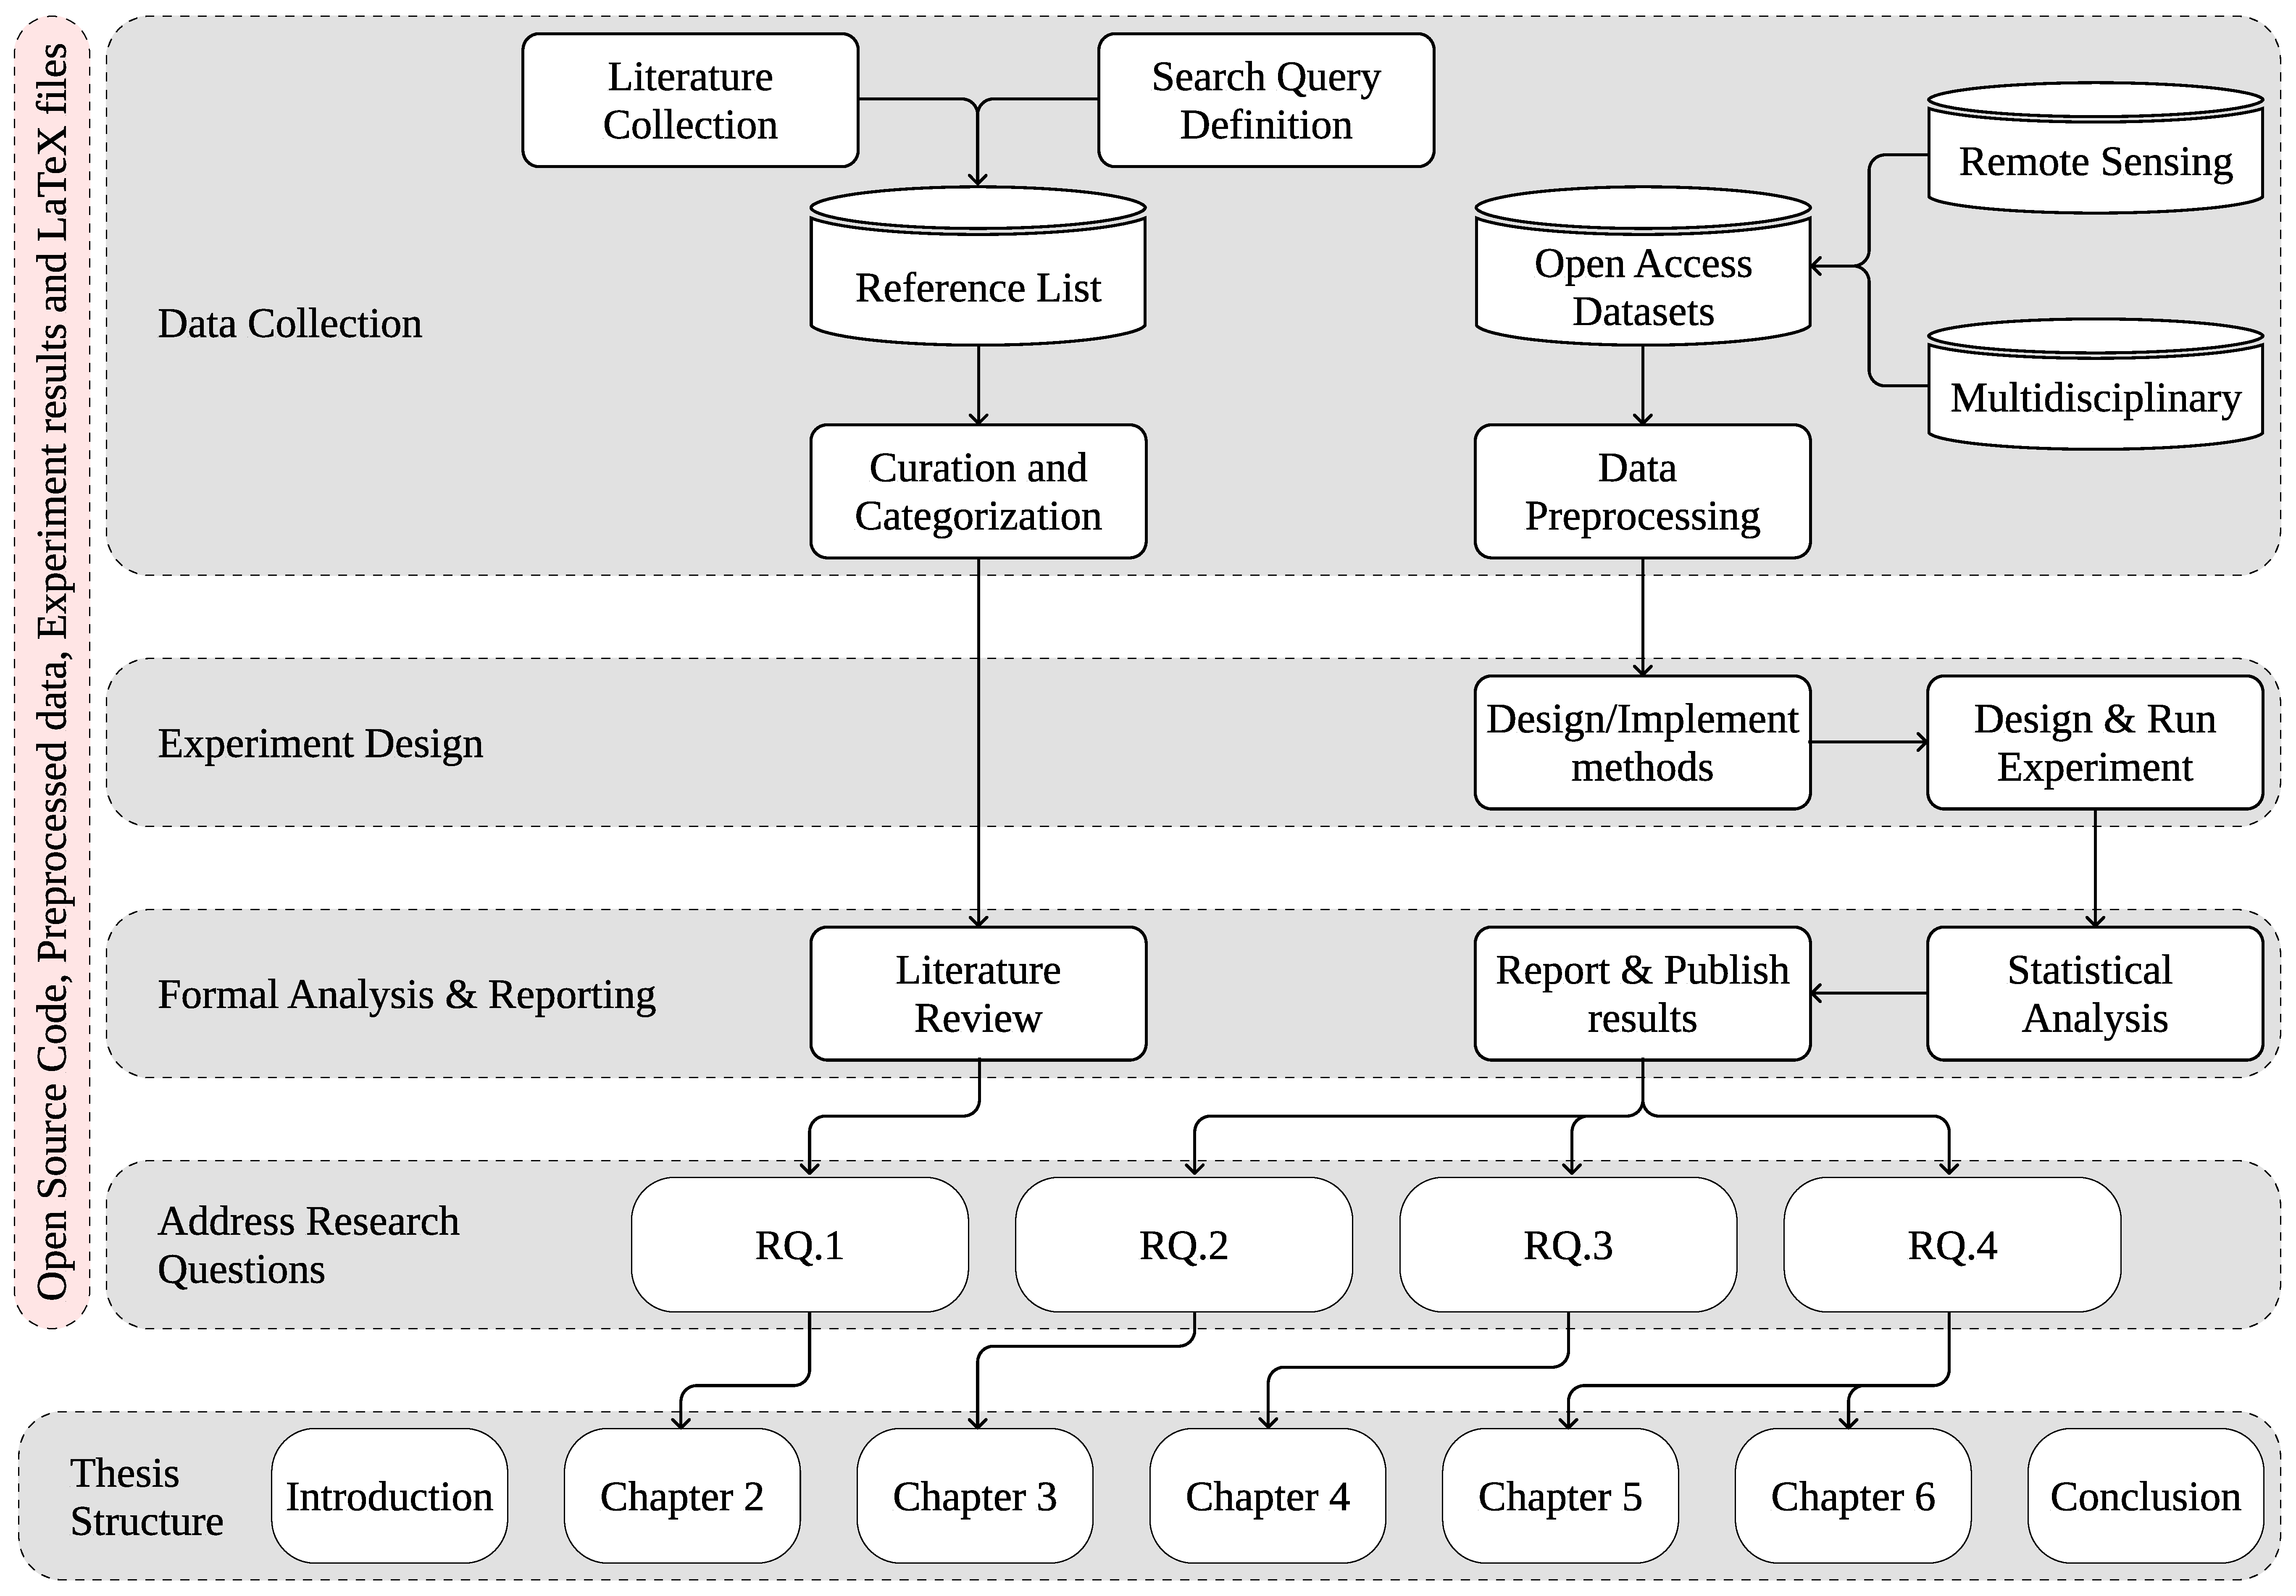
\includegraphics[width=\linewidth]{phd_structure}
    \caption{Planned structure and methodological approach of the doctoral work.
    }~\label{fig:phd_structure}
\end{figure}



\section{Path of Research}

The work developed is organized in different papers of related subjects,
namely AL and imbalanced learning. Every submitted or published research
output is available at
\href{https://github.com/joaopfonseca/publications}{this GitHub repository},
along with the \LaTeX\ scripts, data, source code (for data pulling,
preprocessing, experiments and analysis), experiments' raw outputs and
analysis outputs (figures, tables and diagrams). The current stage of each of
the studies is presented in Table~\ref{tab:studies}.

\begin{table}[ht]
    \centering
    \begin{tabular}{ccm{.55\textwidth}m{.2\textwidth}}
        \toprule
        Chapter & RQ & Study Name                                                        & Current stage  \\
        \midrule
        \ref{chp:data-augmentation-trends} & 1    & Research Trends and Applications 
                                                   of Data Augmentation
                                                   Algorithms                          & Under Review 
                                                                                    (Initial submission)  \\
        \vspace{-.2cm}\\
        \ref{chp:kmeans-smote}             & 2    & Improving Imbalanced Land Cover 
                                                   Classification with K-means SMOTE: 
                                                   Detecting and Oversampling 
                                                   Distinctive Minority Spectral 
                                                   Signatures                          & Published in 
                                                                                         the journal 
                                                                                         Information      \\
        \vspace{-.2cm}\\
        \ref{chp:al-generator-lulc}        & 3    & Increasing the Effectiveness of 
                                                   Active Learning: Introducing
                                                   Artificial Data Generation in 
                                                   Active Learning for Land Use/Land 
                                                   Cover Classification                & Published in 
                                                                                         the journal 
                                                                                         Remote Sensing   \\
        \vspace{-.2cm}\\
        \ref{chp:active-learning-augmentation} & 3 & Improving Active Learning 
                                                   Performance Through the Use of
                                                   Data Augmentation                   & Under Review 
                                                                                       ($2^{nd}$ round)   \\
        \vspace{-.2cm}\\
        n/a & 3     & S$^4$AD-Learning: Self-supervised Semi-supervised Active Deep 
                  Learning                                                          & Work in Progress    \\
        \vspace{-.2cm}\\
        n/a & 4     & Geometric SMOTENC\@: A geometrically enhanced drop-in 
                  replacement for SMOTENC                                           & Work in Progress    \\
        \bottomrule
    \end{tabular}
    \caption{\label{tab:studies}
        Current stage of the planned studies in the scope of the doctoral
        program and PhD grant.
    }
\end{table}

\input{chapters/2-data-augmentation-trends}
\input{chapters/3-kmeans-smote-lulc}
\input{chapters/4-al-generator-lulc}
\input{chapters/5-active-learning-augmentation}
\input{chapters/6-gsmotenc}
\input{chapters/7-moving-forward}

% REFERENCES
\bibliography{references}
\bibliographystyle{ieeetr}
% \bibliographystyle{plain} % Use to validate duplicate references
\addcontentsline{toc}{part}{Bibliography}


% APPENDICES
\appendix
\cleardoublepage%
\addcontentsline{toc}{part}{Appendices}

\chapter{Improving Imbalanced Land Cover Classification with K-means SMOTE:
Detecting and Oversampling Distinctive Minority Spectral Signatures}

\pgfplotstabletypeset[
	begin table=\begin{longtable},
	end table=\end{longtable},
	col sep=comma,
	header=true,
	columns={Dataset,Classifier,Metric,NONE,ROS,SMOTE,B-SMOTE,K-SMOTE},
    string type,
    every head row/.style={before row={\toprule}, after row=\midrule\endhead},
    every last row/.style={after row={\bottomrule
        \caption[Mean cross-validation scores for each dataset.]{%
            Mean cross-validation scores for each dataset.  Legend: IP -
            Indian Pines, KSC - Kennedy Space Center, PC - Pavia Center, PU -
            Pavia University, SA - Salinas A.
        }~\label{tab:cross_validation_scores}
    }}
]{figures/kmeans-smote-lulc/wide_optimal.csv}


\includepdf[pages={3}]{chapters/front-and-back-cover/front-and-back-cover.pdf}
\end{document}
